% !TeX root = ../main.tex
\subsection{问题二：生产过程动态决策}

\subsubsection{任务、信息结构与目标}

问题二要求在给定两类零配件和装配次品率、采购成本、检测成本、装配成本、调换损失及拆解成本后，选择各生产状态下的检测与处置动作。拆解会把零配件送回生产流程，而零配件真实质量在未检测时不可直接观察，因此本问不是一次性的静态组合选择，而是以“当前掌握的质量信息”为状态的序贯决策。

以最终交付一件合格成品为终止条件，并以期望利润或等价的期望成本作为方案比较依据。设从信息状态 $b$ 出发的最小期望成本为 $V(b)$，售价为 $S$，则初始状态下的期望利润为
\begin{equation}
  \Pi=S-V(b_0).
  \label{eq:q2-profit}
\end{equation}
由于同一情形下 $S$ 固定，利润最大化等价于最小化 $V(b_0)$。

\subsubsection{联合信念状态}

设当前持有的零配件真实状态为
\begin{equation}
  \omega_i\in\{N,G,B\},\qquad i=1,2,
  \label{eq:q2-hidden-quality}
\end{equation}
其中 $N$ 表示当前缺少该零配件，$G$ 与 $B$ 分别表示实际合格与实际不合格。企业不能直接观察未检测零配件的 $G/B$ 状态，因此以条件联合分布
\begin{equation}
  b(\omega_1,\omega_2)
  =P(\Omega_1=\omega_1,\Omega_2=\omega_2\mid\mathcal I)
  \label{eq:q2-belief-state}
\end{equation}
作为状态，其中 $\mathcal I$ 汇总已有采购、检测、装配、退换和拆解信息，并满足 $\sum_{\omega_1,\omega_2}b(\omega_1,\omega_2)=1$。初始状态 $b_0$ 集中在 $(N,N)$。

联合分布不能替换为两个独立边际概率。若装配后观察到成品不合格，则“至少一个零配件不合格或装配失败”的信息会使两类零配件质量产生后验相关；丢弃相关性将改变后续检测动作的价值。

\subsubsection{动作、成本与状态转移}

当零配件 $i$ 缺失时，可以购入并检测，检测出不合格件后重复购检直至获得合格件。由几何分布的期望试验次数，成本为
\begin{equation}
  C_i^{T}=\frac{c_i+t_i}{1-p_i},
  \label{eq:q2-buy-test}
\end{equation}
转移后该零配件为已知合格；也可以只支付 $c_i$ 购入而不检测，使其以概率 $1-p_i$ 与 $p_i$ 分别进入未观测的 $G/B$ 状态。

若在手零配件 $i$ 的坏件边际概率大于零，可以支付检测成本 $t_i$ 获取质量信息：检测为合格时将信念条件化到 $\Omega_i=G$；检测为不合格时丢弃该件并把状态置为 $\Omega_i=N$。已经确认合格的零配件不再重复检测。

当两个零配件均在手时，选择装配动作 $A_{y,z}$，其中 $y\in\{0,1\}$ 表示是否检测成品，$z\in\{0,1\}$ 表示不合格成品是否拆解。若两个零配件实际合格，装配仍以概率 $p_f$ 失败；只要至少一个零配件实际不合格，成品必然不合格，因此
\begin{equation}
  P_G(b)=b(G,G)(1-p_f),\qquad P_D(b)=1-P_G(b),
  \label{eq:q2-product-quality}
\end{equation}
一步期望成本为
\begin{equation}
  C(b,A_{y,z})
  =c_a+yt_f+P_D(b)\bigl[(1-y)L+zd\bigr],
  \label{eq:q2-assembly-cost}
\end{equation}
其中，未检测成品在不合格时产生调换损失 $L$，拆解时增加成本 $d$。

成品合格时交付完成。若成品不合格且 $z=0$，零配件随成品报废，状态回到 $b_0$；若 $z=1$，拆解不改变零配件质量，但模型根据“不合格成品”这一观测对回收件信念作贝叶斯更新：
\begin{equation}
  b'(\omega_1,\omega_2)
  =\frac{b(\omega_1,\omega_2)P(D\mid\omega_1,\omega_2)}{P_D(b)},
  \label{eq:q2-bayes-update}
\end{equation}
其中 $P(D\mid G,G)=p_f$，其余情形 $P(D\mid\omega_1,\omega_2)=1$。

\subsubsection{Bellman 最优决策模型}

在每个信念状态 $b$ 下，程序根据缺件、在手件不确定性和可装配性生成动作集 $\mathcal A(b)$。状态--动作价值与 Bellman 最优方程分别为
\begin{align}
  Q(b,a)
  &=C(b,a)+\sum_{b'}P(b'\mid b,a)V(b'),
  \label{eq:q2-q-value}\\
  V(b)
  &=\min_{a\in\mathcal A(b)}Q(b,a),\qquad
  \pi^*(b)=\arg\min_{a\in\mathcal A(b)}Q(b,a),
  \label{eq:q2-bellman}
\end{align}
其中 Bellman 最优方程为有限状态马尔可夫决策过程的标准最优性条件\cite{mdp-puterman,dp-bertsekas}。程序从 $b_0$ 出发遍历可达信念状态，将概率保留六位小数后合并近似相同的状态，再以 Gauss--Seidel 次序执行值迭代，相邻两轮最大状态价值更新量低于 $10^{-10}$ 时停止，并输出状态策略表、各动作 $Q$ 值与最终 Bellman 残差。策略 $\pi^*(b)$ 随信息状态变化，是问题二的求解对象。

\subsubsection{固定决策基准模型}

为量化状态相关策略的增量价值，定义固定决策基准模型。该模型预先固定七个 0-1 决策变量
\begin{equation}
  (x_1,x_2,y,z,r_1,r_2,y_r)\in\{0,1\}^7,
  \label{eq:q2-fixed-strategy}
\end{equation}
其中 $x_i$ 表示首次购件时是否检测零配件 $i$，$y$ 表示首次装配时是否检测成品，$z$ 表示不合格成品是否拆解，$r_i$ 表示拆解回收后是否检测质量不确定的零配件 $i$，$y_r$ 表示拆解后再装配时是否检测成品。给定策略后，按与 5.2.3 节相同的质量传递与成本规则递推期望成本，并枚举全部 $2^7=128$ 个策略取最优。基准结果显示六种情形的最优期望成本分别为 $37.077778$、$44.000000$、$39.411111$、$41.250000$、$40.550000$、$34.321330$ 元。该模型是信念状态 MDP 的受限特例：决策一旦出现新的信息观测便不再调整。

\subsubsection{最优策略与结果分析}

为便于把状态策略还原为业务动作，表~\ref{tab:q2-best-policies}列出从初始状态沿最优策略到首次装配的动作，以及首次装配出现不合格时的下一动作。图~\ref{fig:q2-policy-path}用同一口径比较六种情形，每个格子限定为一个阶段动作：颜色编码动作类别，文字给出具体部件或成品处置方式。

\begin{table}[H]
  \centering
  \caption{六种参数情形下的信念状态最优策略与期望收益}
  \label{tab:q2-best-policies}
  \begin{tabular}{c>{\raggedright\arraybackslash}p{0.28\textwidth}>{\raggedright\arraybackslash}p{0.27\textwidth}rr}
    \toprule
    情形 & 首次装配前动作 & 首次装配及缺陷后动作 & 成本/元 & 利润/元 \\
    \midrule
    1 & 购检部件 1；购部件 2 不检 & 成品不检、缺陷拆解；随后检部件 2 & $37.0778$ & $18.9222$ \\
    2 & 两类部件均购入并检测 & 成品不检、缺陷拆解；随后直接重装 & $44.0000$ & $12.0000$ \\
    3 & 两类部件均购入且不检测 & 检测成品、缺陷拆解；随后检部件 1 & $39.3467$ & $16.6533$ \\
    4 & 两类部件均购入并检测 & 检测成品、缺陷拆解；随后直接重装 & $41.2500$ & $14.7500$ \\
    5 & 购检部件 2；购部件 1 不检 & 成品不检、缺陷拆解；随后检部件 1 & $40.5500$ & $15.4500$ \\
    6 & 两类部件均购入且不检测 & 成品不检、缺陷报废；随后重新购件 & $34.3213$ & $21.6787$ \\
    \bottomrule
  \end{tabular}
\end{table}

\begin{figure}[H]
  \centering
  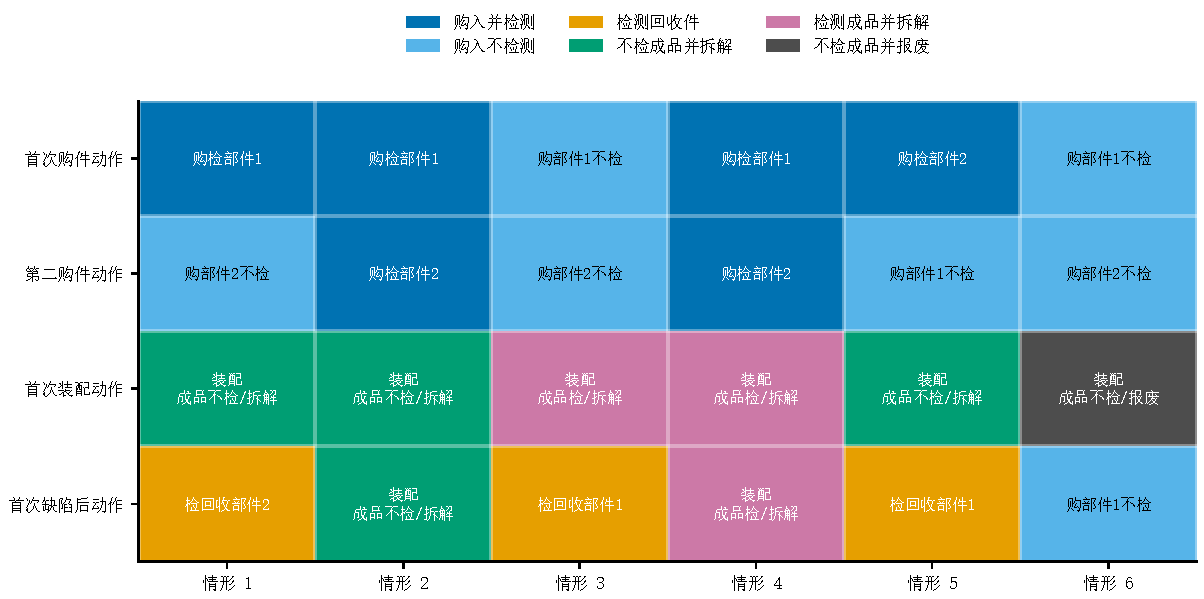
\includegraphics[width=0.98\textwidth]{../../figures/q2/fig_q2_policy_path.pdf}
  \caption{六种参数情形从初始状态到首次缺陷后的最优动作路径}
  \label{fig:q2-policy-path}
\end{figure}

与固定决策基准相比，情形 1、2、4、5 的最优成本在数值容差内一致，情形 6 仅有舍入差异；情形 3 则利用状态相关动作把期望成本由 $39.4111$ 元降为 $39.3467$ 元，改善 $0.0644$ 元：首次对两类部件均不检测，通过成品检测识别不合格成品，拆解后再依据联合后验优先检测部件 1。需要强调的是，信念状态 MDP 的价值主要不在该数值改善，而在于修正固定策略无法利用观测信息的结构性缺陷——成品质量观测会改变后续检测动作的价值，固定 0-1 变量无法表达这一信息反馈。

\subsubsection{收敛性、精度与敏感性检验}

图~\ref{fig:q2-validation}(a) 给出六种情形的值迭代收敛过程，图~\ref{fig:q2-validation}(b) 给出信念概率保留位数对期望成本的影响。

\begin{figure}[H]
  \centering
  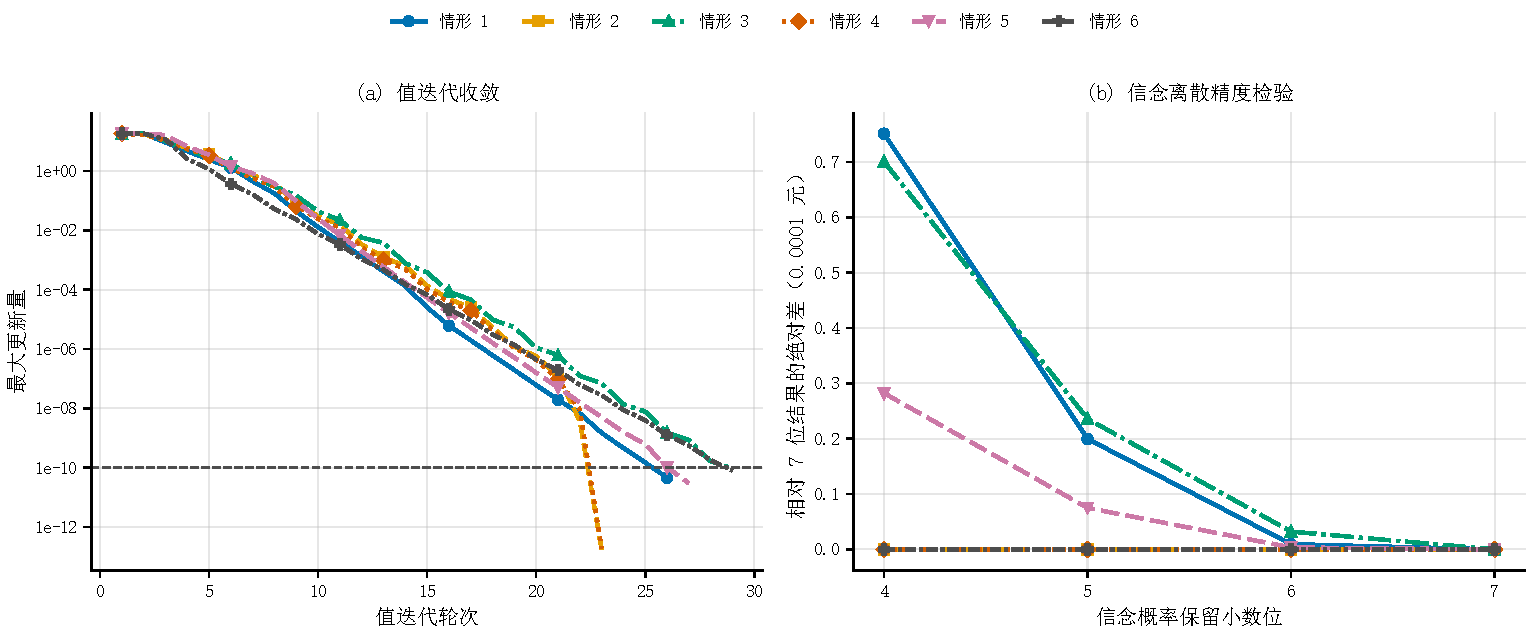
\includegraphics[width=0.98\textwidth]{../../figures/q2/fig_q2_validation.pdf}
  \caption{问题二值迭代收敛与信念状态离散精度检验}
  \label{fig:q2-validation}
\end{figure}

六种情形在 $23$ 至 $29$ 轮内达到停止阈值，最终最大 Bellman 残差为 $2.594\times10^{-11}$；信念概率保留六位小数后合并近似状态，相对七位结果的最大成本差约 $3.2\times10^{-6}$ 元，不改变当前报告精度下的成本或利润结论，详细数值见附录 A.3。进一步分别把三类次品率同步缩放、调换损失和拆解成本乘以 $0.8$ 至 $1.2$，每次只改变一类参数，图~\ref{fig:q2-sensitivity}展示期望利润变化，虚线表示基准参数。

\begin{figure}[H]
  \centering
  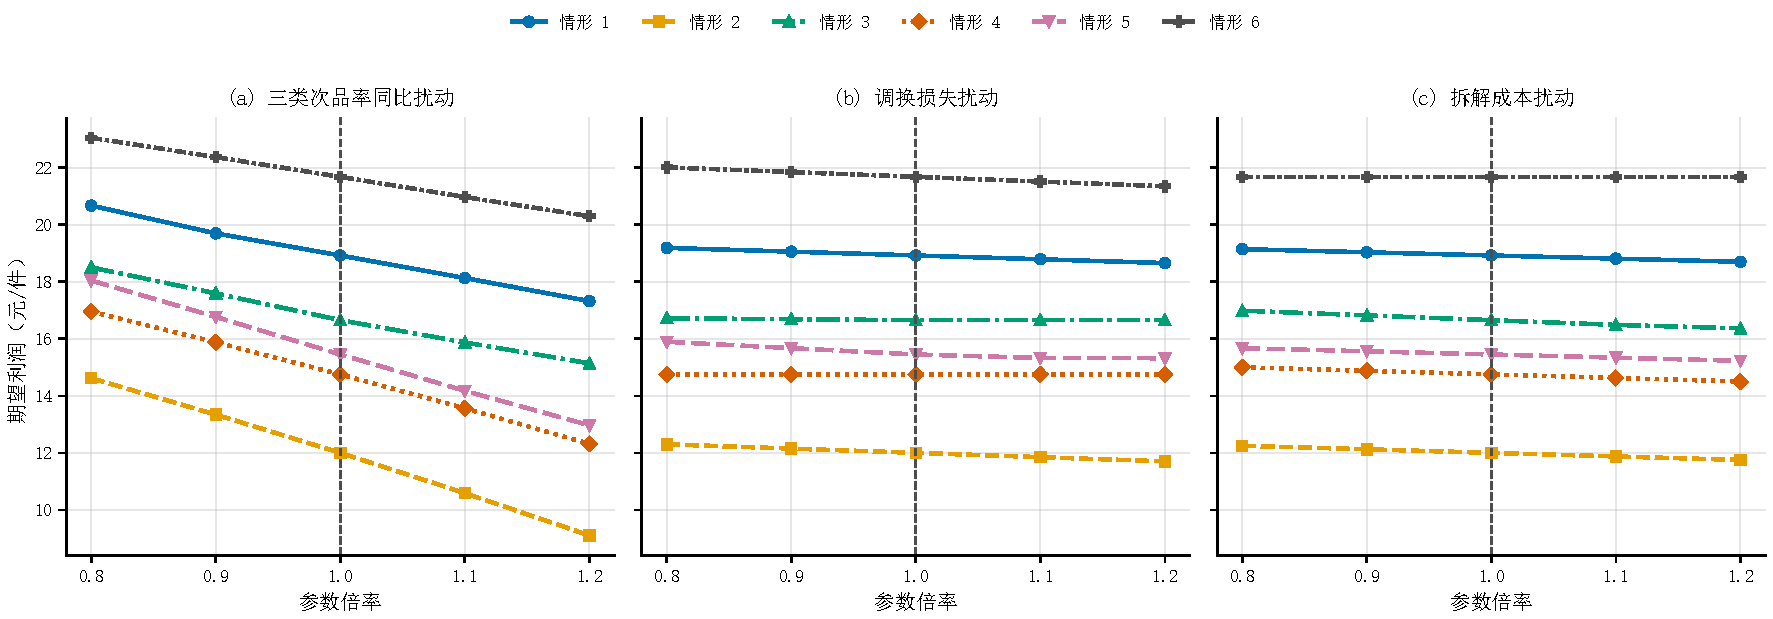
\includegraphics[width=0.99\textwidth]{../../figures/q2/fig_q2_sensitivity.pdf}
  \caption{次品率、调换损失与拆解成本扰动下的期望利润}
  \label{fig:q2-sensitivity}
\end{figure}

次品率扰动对利润的影响最显著：在给定网格内，情形 2 的利润范围为 $9.1053$ 至 $14.6190$ 元，情形 5 为 $12.9673$ 至 $18.0453$ 元，情形 1、3、5、6 出现策略切换；调换损失扰动只使情形 5 在倍率 $1.1$、$1.2$ 时转为检测成品；拆解成本扰动仅在情形 3 倍率 $1.2$ 时触发购检部件 1。图中近似水平的线表示相应最优动作已经隔离了该项损失，而不是参数在模型中被遗漏。

\subsubsection{本问结论}

问题二的输出是信念状态策略而非固定 0-1 向量。六种情形的初始动作、首次装配与缺陷后的后续动作见表~\ref{tab:q2-best-policies}，期望利润依次为 $18.9222$、$12.0000$、$16.6533$、$14.7500$、$15.4500$ 和 $21.6787$ 元。收敛残差、离散精度与三组单因素扰动共同支持上述结果在题目参数及其邻域内的数值可信度；策略切换结果同时表明，超出该参数范围时必须重新求解。
